\documentclass[trackchanges]{aastex631}
\bibliographystyle{aasjournal}

\usepackage[caption=false]{subfig}

\newcommand\natalienote[1]{\textbf{{\color{orange}#1}}}
\newcommand\gullynote[1]{\textbf{{\color{magenta}#1}}}
\newcommand\emilynote[1]{\textbf{{\color{cyan}#1}}}
\newcommand{\Msolar}{M$_{\odot}$}
\newcommand{\Rsun}{R$_{\odot}$}


\begin{document}
\shorttitle{Starspot Coverage on Sub-subgiant S1063}
\shortauthors{Gosnell et al.}

\title{Constraining the Starspot Filling Factor of Active M67 Sub-Subgiant S1063}

\author{Natalie M. Gosnell}
\affiliation{Colorado College, Department of Physics, 14 E. Cache La Poudre St, Colorado Springs, CO 80903}
\author{Michael A. Gully-Santiago}
\affiliation{University of Texas at Austin}
\author{Emily M. Leiner}
\affiliation{CIERA, Northwestern}
\author{Benjamin Tofflemire}
\affiliation{University of Texas at Austin}


\begin{abstract}

We measure the starspots on a sub-subgiant.

\end{abstract}

\keywords{stars: fundamental parameters ---  stars: statistics}


\section{Introduction}\label{sec:intro}
Recent studies illuminate the important role stellar magnetic activity plays in stellar structure. This impact of stellar activity and magnetic fields is seen throughout the Hertzsprung-Russell (HR) Diagram. For example, by biasing isochronal ages of young clusters \citep{somers15}, inflating radii of active M-dwarfs \citep{2010AJ....140.1158T,2010ApJ...718..502M,2019MNRAS.483.1125J}, causing multiple redder turnoffs in stellar clusters \citep{2009MNRAS.398L..11B,2019ApJ...876..113S}, and altering the pulsation modes of red giants \citep{2020A&A...639A..63G}. As our ability to probe the detailed physics of stellar evolution continues to improve we must grapple with the complexities of stellar structure diverging from simpler theoretical expectations due to magnetic activity, which requires careful observational studies of magnetically active systems to test magnetic stellar models.

One example of the impact of magnetic activity is seen in sub-subgiant (SSG) stars, defined to be stars that lie below the subgiant branch on a cluster optical color-magnitude diagram (CMD), but are too red to be main sequence stars. These stars are commonly found in evolved open clusters and globular clusters, with 65 sub-subgiants currently identified across 17 different clusters \citep{geller17}. The majority of sub-subgiant stars are single-lined spectroscopic binaries with short orbital periods of a few days with moderate X-ray luminosities of $10^{30}$ to $10^{31}$ erg s$^{-1}$ \citep[and references therein]{geller17}.

The existence of sub-subgiants cannot be explained with typical single-star stellar evolutionary pathways. Three possible formation scenarios for sub-subgiants were put forth by \citet{geller17} and \citet{leiner17}: mass transfer in a binary system, stripping of a subgiant star envelope through a dynamical encounter, and reduced luminosity as a result of inhibited convection and large starspot covering fractions due to the presence of strong magnetic fields. \citet{leiner17} conclude that the majority of sub-subgiants are likely the result of strong magnetic fields. This interpretation is supported by the presence of H-alpha and X-ray emission and optical variability seen across the known sub-subgiant population \citep{geller17}, all observational signatures of magnetic activity and the presence of starspots.

Ideally, we would directly measure the stellar radius and internal magnetic field strength to calibrate how the star inflates as a function of convective efficiency, thereby explaining the CMD positions of SSGs.  In practice, these quantities are difficult or impossible to measure at the precision required to demonstrate inflation for individual magnetically active systems, though aggregate populations have shown evidence for magnetic inflation \citep{2018AJ....155..225K,2018MNRAS.476.3245J}. Starspots have become a rich observational proxy for gauging the evolutionary state of stars that may be magnetically inflated without needing to estimate magnetic field strengths.


%The portion of the stellar surface covered with starspots is related to the amount of magnetic activity. The mere existence of starspot modulation betrays magnetic activity in stars.  Starspots rupture the otherwise-pristine photospheric boundary conditions that regulate energy loss from stars.  Starspots emit light of their own that can be captured and analyzed to quantify the impact of such boundary condition changes.

A full accounting of starspots requires careful consideration of geometrical degeneracies.  Monochromatic light curves can indicate spotted stars \citep{2014ApJS..211...24M} but only provide a lower limit on the differential spot coverage between the most and least spotted hemispheres. Longitudinally symmetric starspot geometries evade detection in monochromatic lightcurves alone \citep{2019AJ....157...64L}. Disk-integrated covering fractions can be obtained from TiO band observations \citep{oneal96,fang2016,2019AJ....158..101M}. Measuring the spot configuration typically requires Doppler imaging or interferometry studies restricted to only the brightest and most nearby sources \citep{roettenbacher16}.  Testing the next era of stellar activity models requires precision methodologies to measure spot-covering fractions of a larger number of targets, including sub-subgiants.

Starspots emit a spectrum of their own at a lower temperature and with distinct absorption features compared to the ambient photosphere. The observed spectrum is a composite of the spot and photosphere spectra and can therefore be deconvolved. This deconvolution constrains the spot-covering fraction as well as the spot and photosphere temperatures. This is possible by performing a two-temperature probabilistic spectral decomposition using the spectral inference framework \texttt{Starfish} \citep{czekala15}, recently extended to support composite spectra \citep{gullysantiago17}. The resulting spot characterization can be used to anchor light curve information, providing insight into the overall stellar activity level and constraining the long-term spot coverage \citep{neff95}. This strategy only requires high-resolution near-IR echelle spectroscopy and photometric monitoring, dramatically increasing the number of sources for which we can observationally constrain spot-covering fractions.

In this paper we demonstrate the power of this methodology by focusing on a single SSG system, S1063 in the open cluster M67. This system is a prototypical SSG, with an single-lined spectroscopic orbital period of 18.4 days \citep{geller17}, an X-ray luminosity of $1.3\times10^{31}$ erg s$^{-1}$ \citep{vandenberg99}, and a variable light curve in \textit{K2} and ASAS-SN (Section~\ref{sec:K2lightcurve}). \emph{Gaia} DR2 astrometry \citep{2016A&A...595A...1G, 2018A&A...616A...1G} indicates a parallax ($1.17\pm0.025 \;$mas) and proper motion for S1063 (\emph{Gaia} DR2 604921030968952832) consistent with other M67 members  approaching 100\% membership probability \citep{2018ApJ...869....9G}. We present our observational data products in Section~\ref{sec:observations} and subsequent analysis in Section~\ref{sec:analysis}. Our results are given in Section~\ref{sec:results} with Discussion in Section~\ref{sec:discussion}. Finally, our conclusions are outlined in Section~\ref{sec:conclusions}.


\section{Observation and data reduction}
\label{sec:observations}


\subsection{IGRINS observations}
A high resolution spectrum of S1063 was acquired with the $R=45,000$ Immersion Grating Infrared Spectrograph \citep[IGRINS;][]{park14} at UT 2015-04-26 $03^h29^m$ at the $2.7\;$m Harlan J. Smith Telescope at McDonald Observatory.  Eight 600-second individual exposures were acquired in an ABBA nod pattern at an airmass of 1.2.  The sky emission lines and telluric lines were removed with the IGRINS Pipeline Package  \citep[PLP;][]{jaejoonlee16} and a reference A0V star acquired nearby in time and airmass.
The $H-$band spectra exhibited a signal-to-noise ratio of approximately $50$ per pixel.
The $K-$band spectra possessed low $S/N$ and were excluded from further analysis.

\begin{figure*}[ht]
  \centering
  \begin{tabular}{ccccc}
    \subfloat{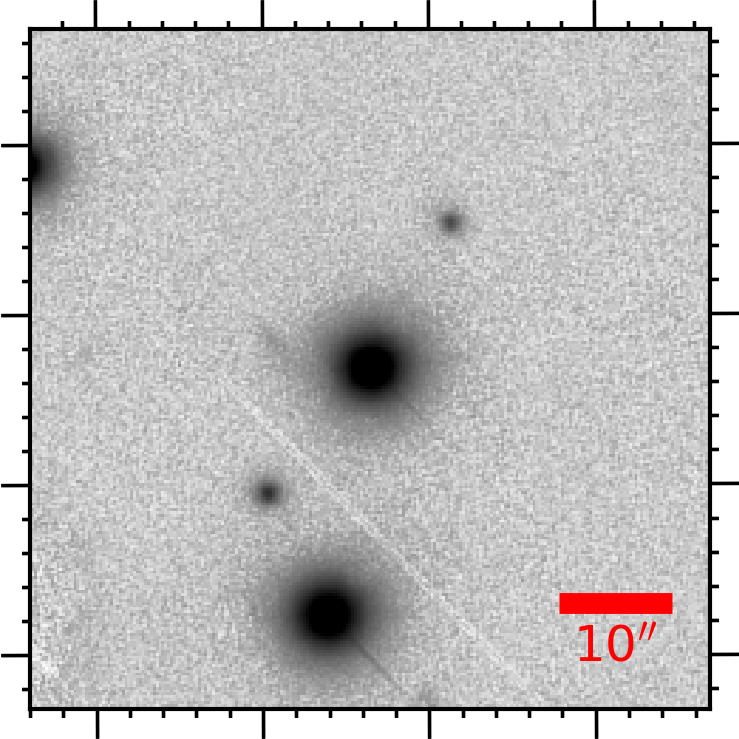
\includegraphics[width=1in]{figures/S1063_60x60arcsec_PS1_g.png}} &
    \subfloat{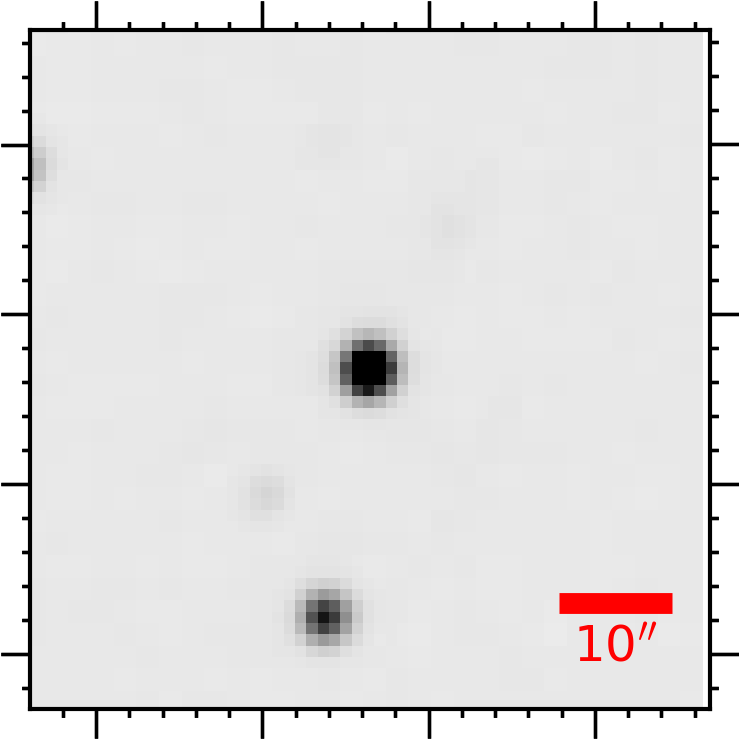
\includegraphics[width=1in]{figures/S1063_60x60arcsec_2M_J.png}} &
    \subfloat{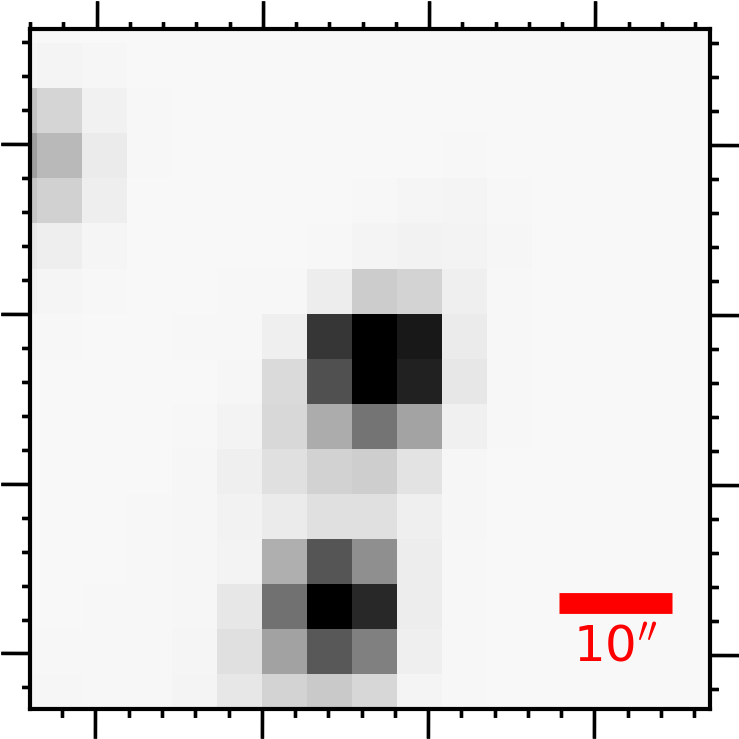
\includegraphics[width=1in]{figures/S1063_60x60arcsec_K2_C5.png}} &
    \subfloat{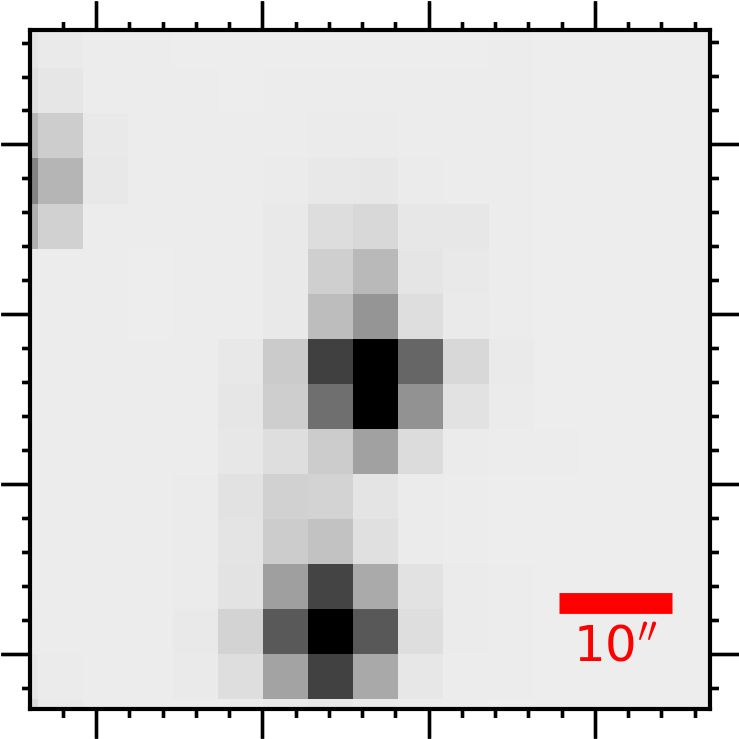
\includegraphics[width=1in]{figures/S1063_60x60arcsec_K2_C16.png}} &
    \subfloat{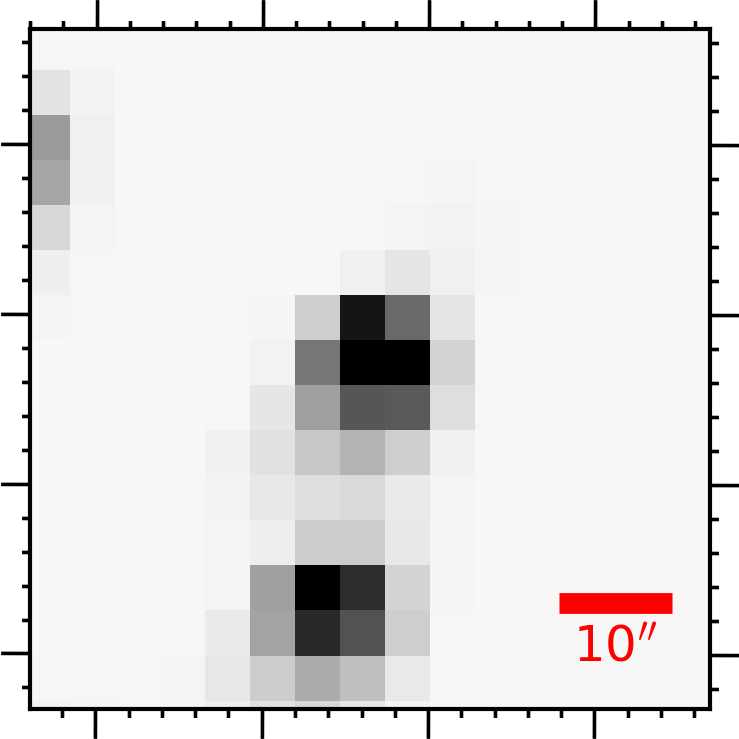
\includegraphics[width=1in]{figures/S1063_60x60arcsec_K2_C18.png}} \\
  \end{tabular}
\caption{Imaging of S1063 in $60'' \times 60''$ postage stamps. \emph{left-to-right:} Pan-STARRS $g$-band co-added image contemporaneous with C16; 2MASS $J-$band; K2 Campaigns 5, 16, 18 from Full Frame Images.  S1063 is sufficiently separated from nearby sources in the coarse \emph{Kepler} imaging.}
\label{fig:imaging}
\end{figure*}

\subsection{K2 superstamp lightcurves}
The \emph{Kepler} spacecraft targeted S1063 (EPIC 211414597) during the \emph{K2} mission \citep{howell14} in Campaigns 5, 16, 18 as part of the M67 superstamps.  The instrumental point spread function (PSF) of S1063 fell entirely within the oversized K2 target pixel files in Campaign 5 (K2 Custom Aperture ID 200008674, channel 13) and Campaign 18 (K2 Custom Aperture ID 200233338).  Aperture photometry was conducted with interactively-assigned custom apertures using the \texttt{lightkurve.interact()} feature \citep{geert_barentsen_2019_2565212}. The apertures were chosen to minimize flux-loss out of the aperture due to spacecraft-induced image motion, while avoiding low-$S/N$ pixels and the wings of adjacent PSFs.  The Campaign 16 source PSF overlapped the edge of Custom Aperture ID 200200534, therefore a mosaic of adjacent superstamps was assembled before conducting aperture photometry.
We detrended motion-induced image artifacts with the Self Flat Field algorithm \citep{vanderburg14} implemented in \texttt{lightkurve}.  Postage stamp images are shown in Figure \ref{fig:imaging}.


\subsection{Ground-based photometric monitoring}
We retrieved All-Sky Automated Survey for Supernovae \citep[ASAS-SN;][]{shappee14} lightcurves from the Sky Portal \citep{2017PASP..129j4502K}.  The lightcurves contained 758 epochs of $V$-band photometry spanning 2013-2018 (source ASASSN-V J085113.44+115139.7) and 823 epochs of $g$-band photometry spanning mid-2017--2018.  The $\sim8''$ ASAS-SN pixels may cause some PSF blending of the nearby-albeit-fainter source seen at the bottom of Figure \ref{fig:imaging}.  The pixel images were not available to evaluate the extent of blending.

\subsection{Inter-campaign relative photometry with K2 Full Frame Images}\label{sec:K2lightcurve}

Stellar activity cycles on S1063 can secularly change the stellar brightness on timescales comparable to the separation of the three campaigns of \emph{K2} observations.  The comparison of flux levels among repeated \emph{K2} campaigns requires accounting for detector responsivity degradation on these same timescales.  The absolute sensitivity of the \emph{Kepler} detector pixels decay at $\sim1 \%\;\textrm{yr}^{-1}$ due to sudden pixel sensitivity dropouts and other environmental lifetime factors \citep{montet17}.

To account for sensitivity changes, we calibrate the system-integrated throughput for \emph{Kepler} detector channels including the M67 field for Campaigns 5, 16, and 18. We measure aperture photometry for approximately 2000 isolated reference stars from the Full Frame Images, keeping only those stars that were observed in all three campaigns. Compared to Campaign 5, the reference stars have a median flux of $93.9\pm4.2\%$ in Campaign 16 and a median flux of $98.2\pm2.8\%$ in Campaign 18. Campaigns 5 and 18 were observed on the same detector channel while a different detector channel was used for Campaign 16, therefore these offsets are not a significant measure of detector degradation across campaigns. We use a Lomb-Scargle periodogram on each campaign independently and recover the same dominant period of 23.5 days in all three campaigns. The phase-folded light curves and periodograms are shown in Figure~\ref{fig:periodogram}.



\begin{figure*}[ht]
    \centering
    \begin{tabular}{cc}
      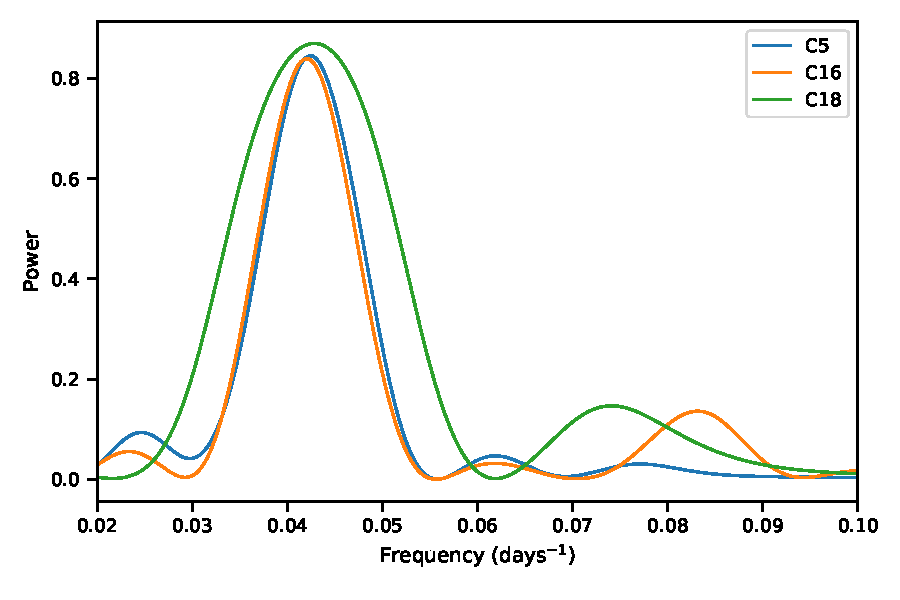
\includegraphics[width=3in]{figures/AllCampaigns_Periodogram.pdf}   & 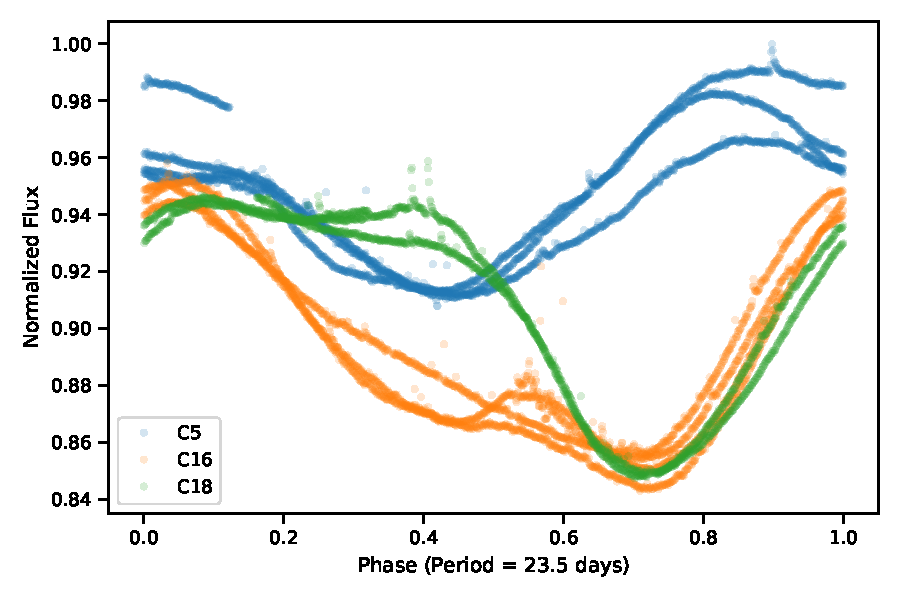
\includegraphics[width=3in]{figures/AllCampaigns_Phased_Lightcurve.pdf}  \\
    \end{tabular}
    \caption{On the right, a Lomb-Scargle Periodogram of the light curve for each \emph{K2} campaign and on the left, the corresponding phased \emph{K2} light curves. The average period associated with maximum power across all three campaigns is P = 23.5 days.  }
    \label{fig:periodogram}
\end{figure*}


\begin{figure*}[ht]
  \centering
  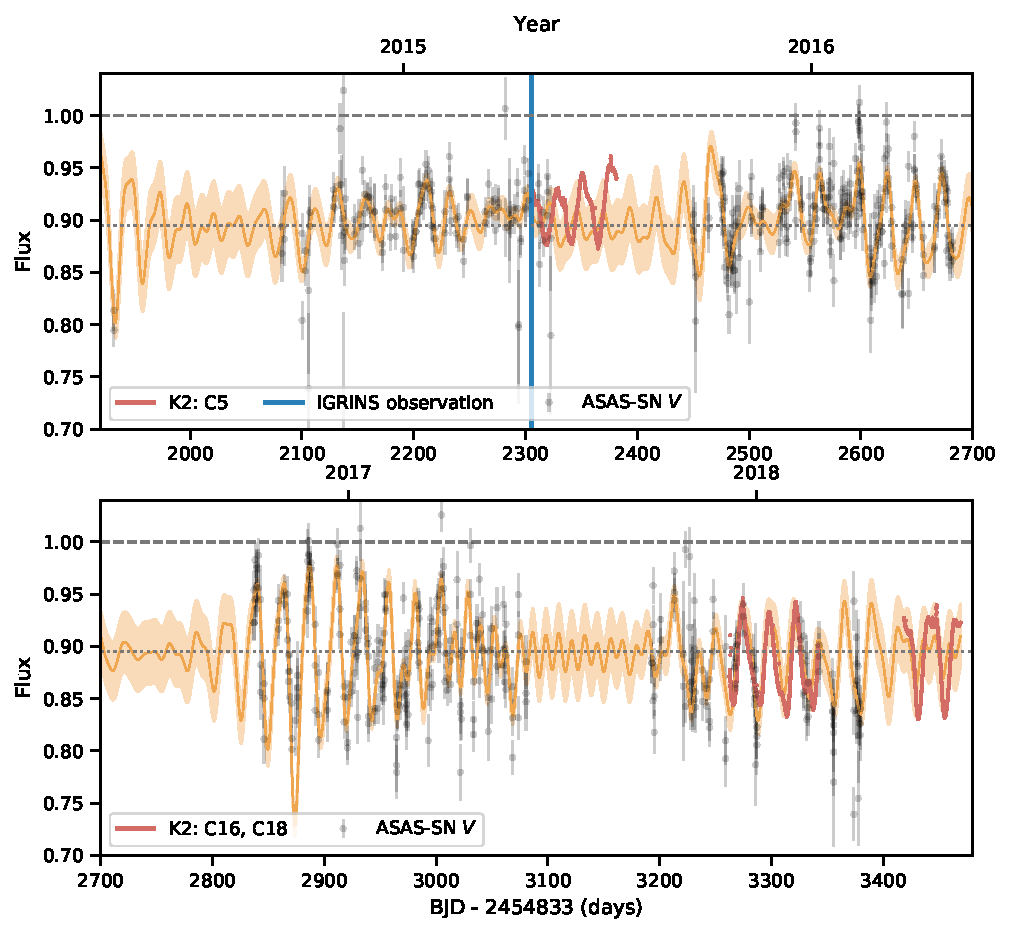
\includegraphics[width=0.95\textwidth]{figures/2020_K2_ASASSN_lcurve_2panel.pdf}
\caption{Four year lightcurve for S1063, normalized to a maximum flux of 1.00 as denoted by the gray dashed line. The mean flux of 0.895 is shown with the gray dotted line.  \emph{K2} Campaigns 5, 16, and 18 (densely-sampled red points) and ASAS-SN $V-$band (coarsely-sampled gray points) show approximately $5-17\%$ peak-to-valley photometric variations indicative of secularly evolving surface coverage of starspots.  The orange line shows a damped, driven harmonic oscillator \texttt{celerit\`e} model \citep{2017AJ....154..220F} trained on the \emph{K2} and ASAS-SN data, and then applied to the noisy ASAS-SN points. A standard-error uncertainty band is shown in shaded orange. The vertical blue bar in mid-2015 indicates the epoch of IGRINS data acquisition, which shows an approximate $8\%$ flux deficit compared to the global maximum flux in early 2017.}
\label{fig:lightcurve}
\end{figure*}


\section{Analysis}
\label{sec:analysis}

%INTRO TEXT:
%Starspots emit a spectrum of their own at a lower temperature and with distinct absorption features compared to the ambient photosphere. The observed spectrum is a composite of the spot and photosphere spectra and can therefore be deconvolved. This deconvolution constrains the spot-covering fraction as well as the spot and photosphere temperatures. This is possible by performing a two-temperature probabilistic spectral decomposition using the spectral inference framework \texttt{Starfish} \citep{czekala15}, recently extended to support composite spectra \citep{gullysantiago17}. The resulting spot characterization can be used to anchor light curve information, providing insight into the overall stellar activity level and constraining the long-term spot coverage \citep{neff95}. This strategy only requires high-resolution echelle spectroscopy and photometric monitoring, dramatically increasing the number of sources for which we can observationally constrain spot-covering fractions.

Constraining starspot covering fraction for stars such as S1063 requires a careful combination of light curve interpretation and spectral analysis using spectral decomposition tools such as \texttt{Starfish} \citep{czekala15} to benchmark epochs of starspot coverage in long-term photometric monitoring.

\subsection{Joint modeling of ASAS-SN and \emph{K2} Lightcurves}
Characterizing the long-term behavior of S1063 requires connecting and comparing photometry information from different missions, in this case ASAS-SN and \emph{K2}. To accomplish this task we jointly modeled the ASAS-SN and \emph{K2} lightcurves as a damped, driven Simple Harmonic Oscillator (SHO) Gaussian Process (GP) with \texttt{celerit\`e} \citep{2017AJ....154..220F}, revealing periodicity and secular changes in flux levels over a multi-year timeframe.  This strategy offers flexibility to cope with windowing effects and the high dynamic range in data sampling and quality available across ASAS-SN and \emph{K2}.  The ASAS-SN $V$-band and \emph{K2} photometric band share significant overlap and are treated as the same for this analysis.

We tuned a two-period GP model with the harmonic component possessing roughly half the period $P_H\sim12.5\;\mathrm{d}$ of the fundamental period $P_0=23.5\;\mathrm{d}$.  The harmonic overtone frequency can be seen by eye in Figure \ref{fig:lightcurve}, as the \emph{K2} lightcurves appear more complex than a pure sine wave.  Each periodic GP term also possessed a correlation amplitude and SHO quality factor which we consider nuisance parameters for the purpose of this fitting.  We found broadly consistent values when \emph{K2} lightcurves were fitted on a per-campaign basis.  We then fit the three campaigns \emph{simultaneously} in the following way.  We set the overall vertical registration of the \emph{K2} lightcurves such that the ASAS-SN and Campaign 16 trends match, since M67 was contemporaneously observable from the ground for the entire duration of K2 Campaign 16. The uncertainty in the inter-campaign offsets calculated in Section~\ref{sec:K2lightcurve} is larger than the internal precision of the \emph{K2} photometry, so we adjust the Campaign 5 data within the offset uncertainty to match the approximately one week of temporal overlap with ASAS-SN.  We added an additional non-periodic secular trend GP component to capture the campaign-to-campaign mean-level variation, also considered a nuisance parameter.

Finally, we evaluated the trained GP model at the location of the ASAS-SN photometry, and at windows lacking data altogether.  This trend appears in Figure \ref{fig:lightcurve} as the dark orange line with an orange shaded standard confidence region.  This trendline guides the eye to see broad secular changes to the amplitude encoded in the noisy ASAS-SN data, with a global maximum peak-to-valley amplitude of 17\% occurring near 2017 January, and global minimum peak-to-valley of 3\% occurring shortly before the IGRINS measurement.



\subsection{IGRINS two-temperature spectral decomposition}

Even a single epoch of IGRINS observations provides an opportunity to constrain the spot covering fraction of S1063 that can be used as a benchmark for interpreting the long-term flux variation apparent in Figure~\ref{fig:lightcurve}. We performed a two-temperature probabilistic spectral decomposition on the IGRINS $H$-band spectrum.  We applied the spectral inference framework \texttt{Starfish} \citep{czekala15}, recently extended to support composite spectra comprised of mixtures of two distinct photospheric components \citep{gullysantiago17}.  Here, the two temperature components are labeled as $T_{\mathrm{spot}}$ and $T_{\mathrm{amb}}$ for the starspot and ambient photospheric emission, respectively, with a filling factor $f$ defined as the ratio of disk-integrated projected surface area of the spot groups to the projected area of the star.

We employed the \texttt{PHOENIX} pre-computed synthetic model grid \citep{husser13} with grid ranges of $3000 < T_{\mathrm{eff}} \; (\textrm{K}) < 5300 $, $3 < \log{g \;(\textrm{cm/s})}  < 4 $, and $ -0.5 <  [\mathrm{Fe}/\mathrm{H}] <0.5$.  We trained the spectral emulator \citep{czekala15} on this grid range, while preserving the absolute model mean fluxes to enable accurate flux comparison between two spectra of disparate characteristic temperatures.  This new approach offers improved accuracy over the scalar flux interpolated approach introduced in Appendix A of \citet{gullysantiago17}, especially for such a large dynamic range in effective temperature.  The spectral emulator approach also propagates the uncertainty attributable to the coarsely sampled \texttt{PHOENIX} models.

The pre-defined grid ranges place uniform priors over their domain.  Additionally, a threshold of 4500 K separated the allowed domains for the spot and ambient temperatures, yielding uniform priors $3000 < T_{\mathrm{spot}} \; (K) < 4500 $ and $4500 < T_{\mathrm{amb}} \; (K) < 5300$.

\subsubsection{MCMC convergence and posterior predictive checks}

Each IGRINS $H$-band spectral order was fit independently, yielding over 20 individual sets of MCMC posteriors.  We employed \texttt{emcee} \citep{foreman13} with 5000 samples and 40 walkers, spot-checking the MCMC chains for signatures of steady-state posterior probability distributions suggestive of convergence.  Some orders did not pass our convergence criteria, usually due to poor initialization of nuisance parameters or over-fitting.  Furthermore, the radial velocity $v_z$ and projected rotational broadening $v\sin{i}$ were spot-checked to verify both consistent values among spectral orders as well as posterior distributions indicative of information-rich spectral orders.  Some relatively feature-free spectral orders did not offer enough constraining power to derive meaningful results in the face of multiple sources of degeneracy.  Collectively, these discrepant or uninformative spectral orders were removed from future analysis, yielding a total of nine preserved spectral orders, shown in Figure \ref{fig:IGRINS_spectra3x3}. All spectral orders were consistent with a $v\sin{i}=10 \;\mathrm{km/s}$, with typical per-order $1-\sigma$ uncertainties of $0.2-1.0 \;\mathrm{km/s}$.  The per-order estimates for radial velocity were all consistent with $v_z=44\;\mathrm{km/s}$ at the measurement epoch, uncorrected for barycentric motion.

\begin{figure*}[ht]
 \centering
 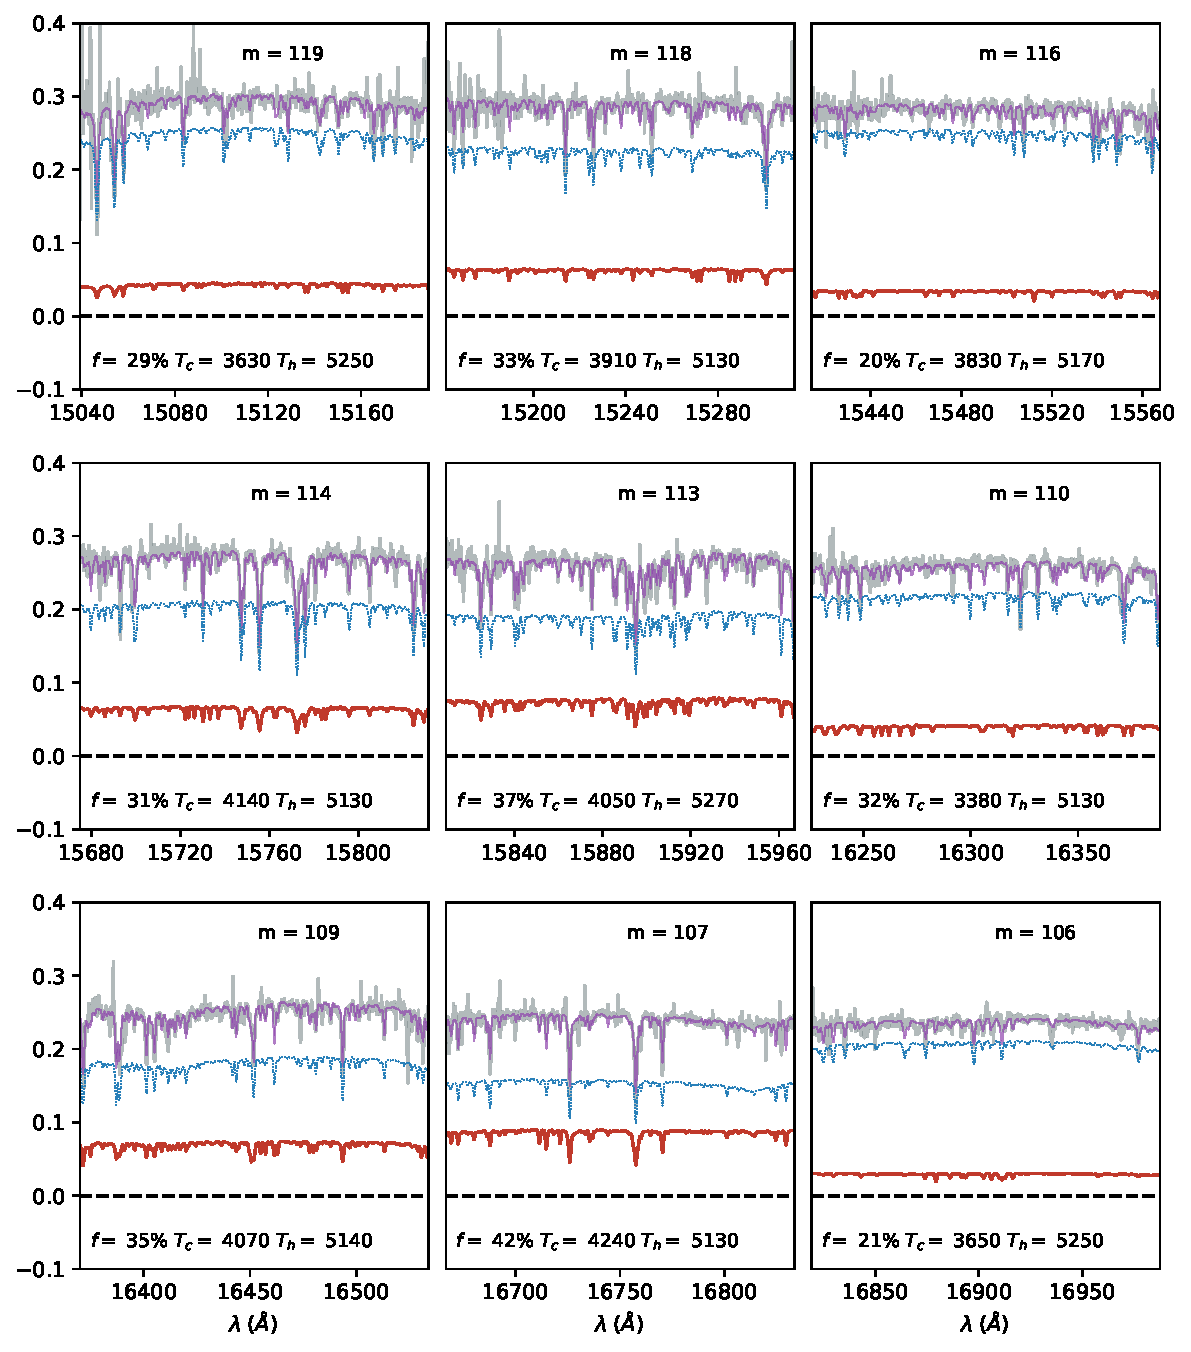
\includegraphics[width=0.90\textwidth]{figures/H_band_spectra_3x3.pdf}
 \caption{Nine $H-$band IGRINS echelle orders showing two-component spectral decomposition of collective starspot photospheric emission, labeled with the corresponding order number $m$.  The starspot spectrum (thick red line) and ambient photosphere spectrum (dotted blue line) combine to form the composite spectrum (solid purple line) that resembles the observed spectrum (thick gray line).  The starspot and ambient components can share similar spectral structure, leading to a range of filling factors and temperatures ranges with nearly equivalent composite spectra; here we present a single random draw from the MCMC posterior, not a ``best fit''.  The cool and hot temperatures $T_{\textrm{s}}$ and $T_{\textrm{amb}}$ for each draw show variety consistent with the fitting uncertainty. The corresponding spot filling factor, $f_{\textrm{s}}$, is also shown for each specific random draw. Unexplained spectral structure and over- and under- fitting of spectral lines arises from a combination of PHOENIX model imperfections, possible magnetic Zeeman broadening, and other model mis-specifications.}
 \label{fig:IGRINS_spectra3x3}
\end{figure*}

%\subsubsection{Consistency of stellar characterization}
%Vsini is similar to before and radial velocity is what we expect given orbital phasing (NEED TO DO THE PHASING).


%TODO: Analysis of near-IR flux contribution from binary companion
%TODO: Limits on companion types


\section{Results}
\label{sec:results}

\subsection{Spot temperature and filling factor}
\label{sec:starfishresults}
Using the \texttt{Starfish} spectral inference results we investigate the joint constraints on spot temperature and filling factor, marginalized over all other uncertainties in stellar properties and fitting hyper-parameters (such as \texttt{Starfish}-derived Gaussian Process correlation length and amplitude and continuum fitting polynomials). In Figure~\ref{fig:tspot_fillingfactor3x3} we show 2-dimensional posterior distributions of filling factor and spot temperature of the last 1000 samples thinned by a factor of 10 from all 40 \texttt{emcee} walkers for the nine orders with accepted fits. The orders show broad agreement between spot temperature and filling factor. Across all nine orders, the median filling factor value is 32\% with a standard deviation of 7\%, with a corresponding spot temperature of $4000 \pm 200$ K. The ambient photosphere temperature associated with this spot signature varies from order-to-order and is broadly consistent with a range of temperatures between 5000 K and 5300 K, with a best guess value of 5200 K.  These values are broadly consistent with a spectroscopic temperature of 5000 K for S1063 determined by \citet{mathieu03} determined from visible-wavelength spectra.  Visible wavelength spectra principally perceive the ambient photosphere, due to the near-zero starspot contrast at those wavelengths.  Therefore the most reliable ambient photosphere estimate likely stems from the visible-based measurement, and not our near-IR-based estimate.

\subsubsection{Light curve interpretation}
The ASAS-SN and \textit{K2} Campaign 5 data of S1063 (Figure~\ref{fig:lightcurve}) indicate that the IGRINS observation was coincidentally acquired near its modest local maximum at an overall flux level of 91.2\%. This is close to the overall 89.5\% mean flux level, where the 100\% flux level is equal to the global maximum over the four-year period covered by ASAS-SN and \textit{K2}. The lightcurve exhibits relatively modest variability at the time of the IGRINS observations with merely 3\% peak-to-valley variation compared to its global largest variation of almost 17\% as observed around 2017 January.

For a first-order interpretation of light curve amplitudes, we posit that the lightcurve is starspot-dominated as opposed to facula-dominated.  Under this assumption, minimum light corresponds to the largest blockage of ambient flux and therefore the largest starspot coverage on the instantaneous hemisphere projected towards the observer \cite{basri18}.  Maximum light corresponds to the moments with the least---\emph{but not necessarily zero}---starspot coverage.

If S1063 was spot-free at the time of the global lightcurve maximum the epoch of IGRINS observation would correspond to starspots blocking 8.8\% of the total instantaneous stellar flux (100\% $-$ 91.2\% $=$ 8.8\% blocked flux at the time of observation), assuming non-emitting starspots. However, starspots are emitting and effectively filling in some of the light that is ``blocked''.  This non-zero starspot emission demands that the spot covering fraction must be greater than 8.8\% at the time of the IGRINS observation. Adopting an ambient photosphere temperature of 5200 K and a spot temperature of 4000 K, the projected spot coverage of S1063 must be at least 13\% to account for the 8.8\% flux loss in the $V$-band.

This 13\% spot coverage is a minimum value based on an assumption that the maximum lightcurve flux results from an un-spotted star. Our spectral inference results indicate the spot coverage at the time of the IGRINS observation was, in fact, 32\%. This suggests that at maximum light over this 4-year period the spot coverage of S1063 was approximately 20\%, and not zero as a first-order interpretation of the light curve would imply.

The presence of starspots at the light curve maximum acts as a starspot baseline for interpreting the lightcurve. Over the four years shown in Figure~\ref{fig:lightcurve}, the average flux variation is approximately 5\%, corresponding to an average spot covering fraction variation from each observed hemisphere of $\pm$8\%. The lightcurve exhibits a global flux minimum 10\% lower than the flux at the time of the IGRINS observation, requiring a spot filling factor close to 45\% on the projected hemisphere at that time.

We therefore determine that over the time period from 2014--2018 S1063 has possessed a range of 20--45\% coverage fraction of spots, with an average close to 30\%. The IGRINS observation occurring near the mean global flux level fortuitously allows a robust characterization of the average state of S1063. These numbers possess formal uncertainties in the few percent range, and additional uncertainties from our reliance on spectral models.  But broadly speaking, our result is firm under our assumptions --- S1063 has a large persistent starspot population that ebbs and flows in its longitudinal symmetry, resulting in variation in the peak-to-valley modulation, but always possesses an approximately 30\% spot covering fraction.

\begin{table}[]
\label{tab:s1063parameters}
\caption{S1063 Surface and Stellar Parameters}
\begin{tabular}{llcccc}

  &         & Spot temp  & Filling factor & Ambient temp & Radius  \\
   &        &  (K) & (\%) &  (K) & ($R_{\odot}$) \\ \hline
\multicolumn{3}{l}{\textit{Spectroscopic Constraints:}}  \\
\phantom{EEE} & This work     & $4000\pm200$  & $32\pm7$    & 5200 &   3.7--4.6$^{a}$     \\
& \citet{mathieu03} &  ...    &  ...    &     5000    &  2.4  \\
\multicolumn{3}{l}{\textit{Photometric Constraints:}} \\
& Gaia SPOTS models$^{b}$  &   4100   &  51  &   5100  &   3.0  \\
& 2MASS SPOTS models &   4200   & 85    &   5300  &    3.1    \\
& \citet{leiner17} & ... & ... & 4500$^{c}$ & 2.8--3.1 \\
& & 3500$^{d}$ & 40 & 4750 & 3.4 \\
\hline
\multicolumn{6}{l}{$^{a}$$R \sin i$, determined from $v\sin i$, see Section~\ref{sec:radius}} \\
\multicolumn{6}{l}{$^{b}$Section~\ref{sec:model_comparison}, from \citet{somers20}.} \\
\multicolumn{6}{l}{$^{c}$Unspotted model.} \\
\multicolumn{6}{l}{$^{d}$Model assuming 40\% spot coverage with a spot temperature contrast of $\sim$1000 K.}
\end{tabular}
\end{table}


 \begin{figure*}[ht]
   \centering
   \begin{tabular}{ccc}
     \subfloat{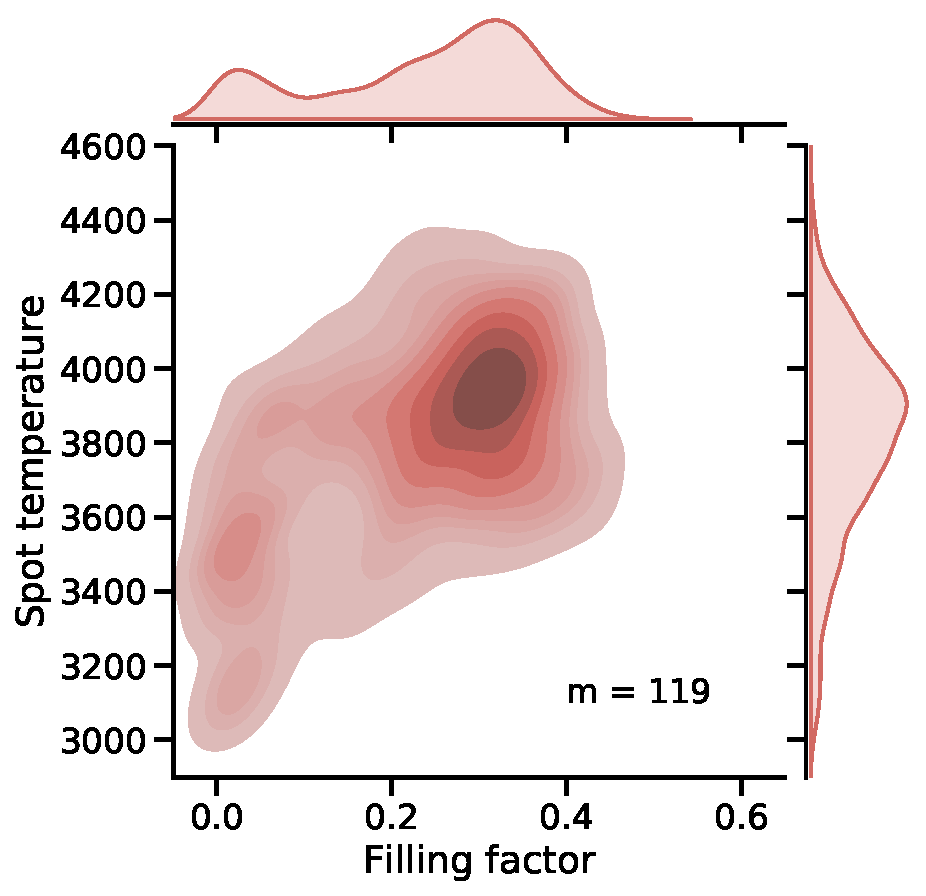
\includegraphics[width=2in]{figures/H_band_Tspot_fillingfactor_m119_new.pdf}} &
     \subfloat{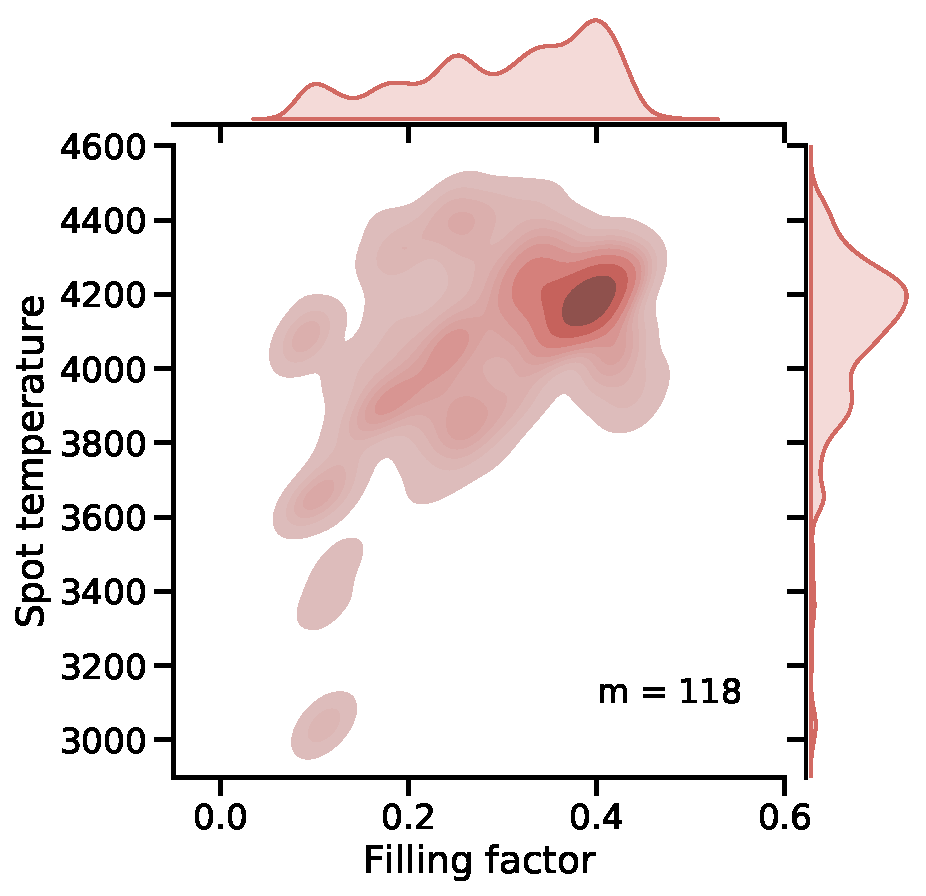
\includegraphics[width=2in]{figures/H_band_Tspot_fillingfactor_m118_new.pdf}} &
     \subfloat{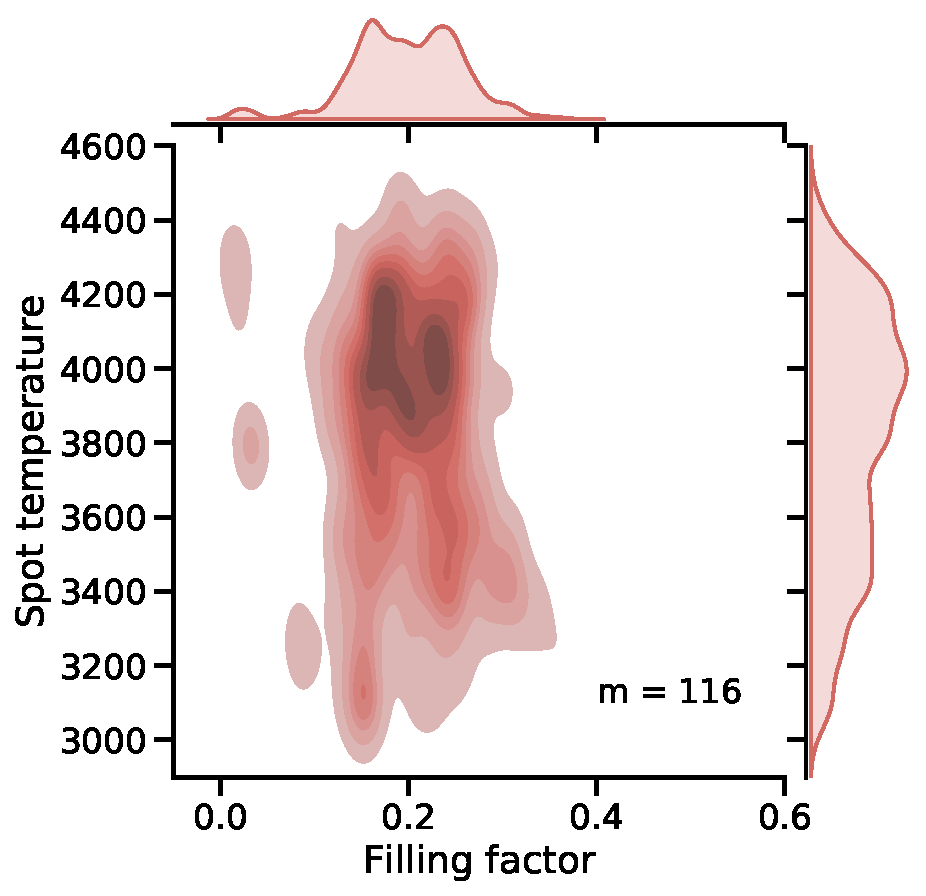
\includegraphics[width=2in]{figures/H_band_Tspot_fillingfactor_m116_new.pdf}} \\
     \subfloat{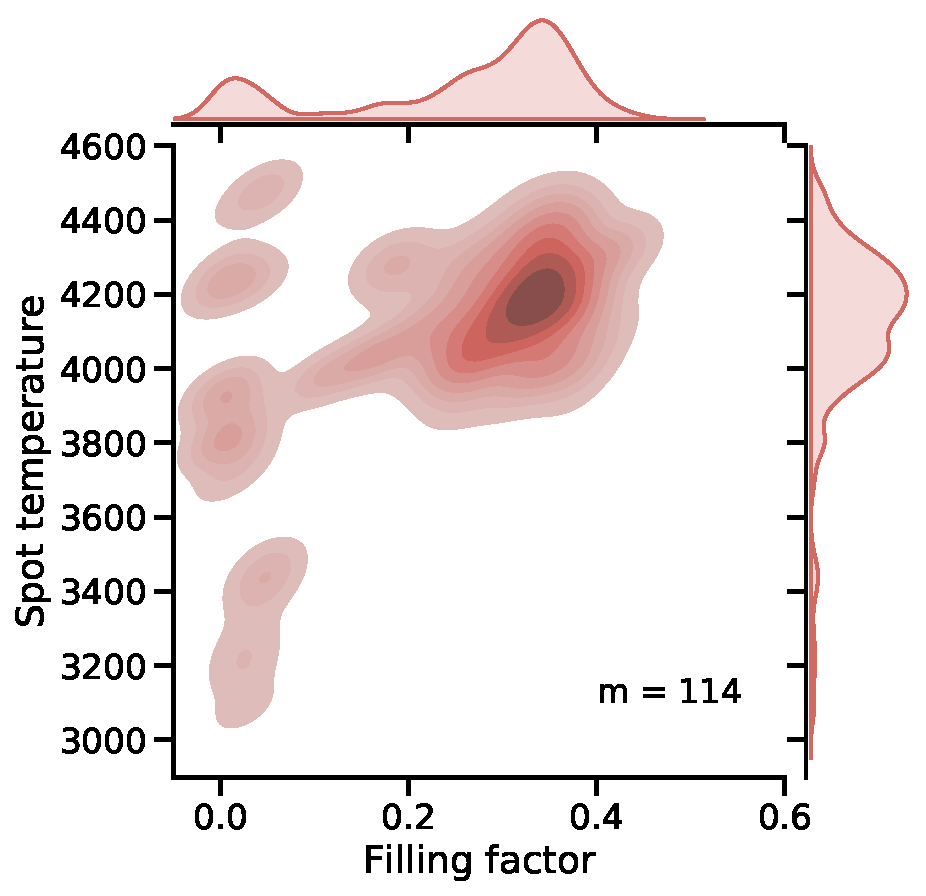
\includegraphics[width=2in]{figures/H_band_Tspot_fillingfactor_m114_new.pdf}} &
     \subfloat{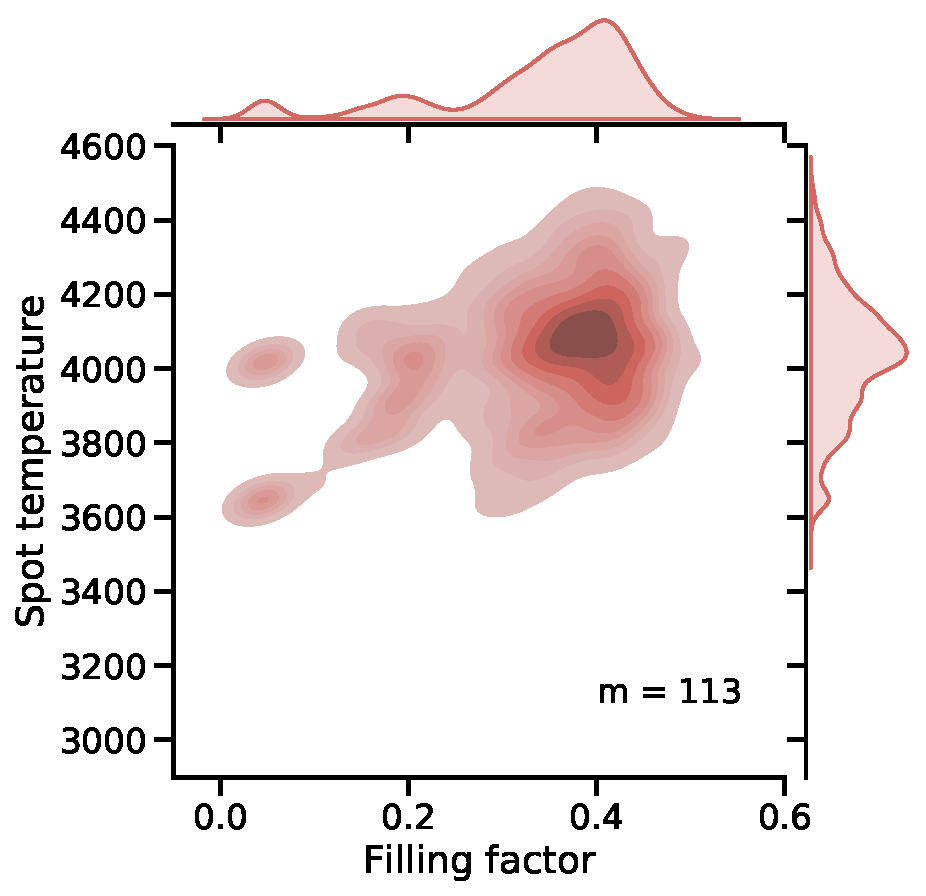
\includegraphics[width=2in]{figures/H_band_Tspot_fillingfactor_m113_new.pdf}} &
     \subfloat{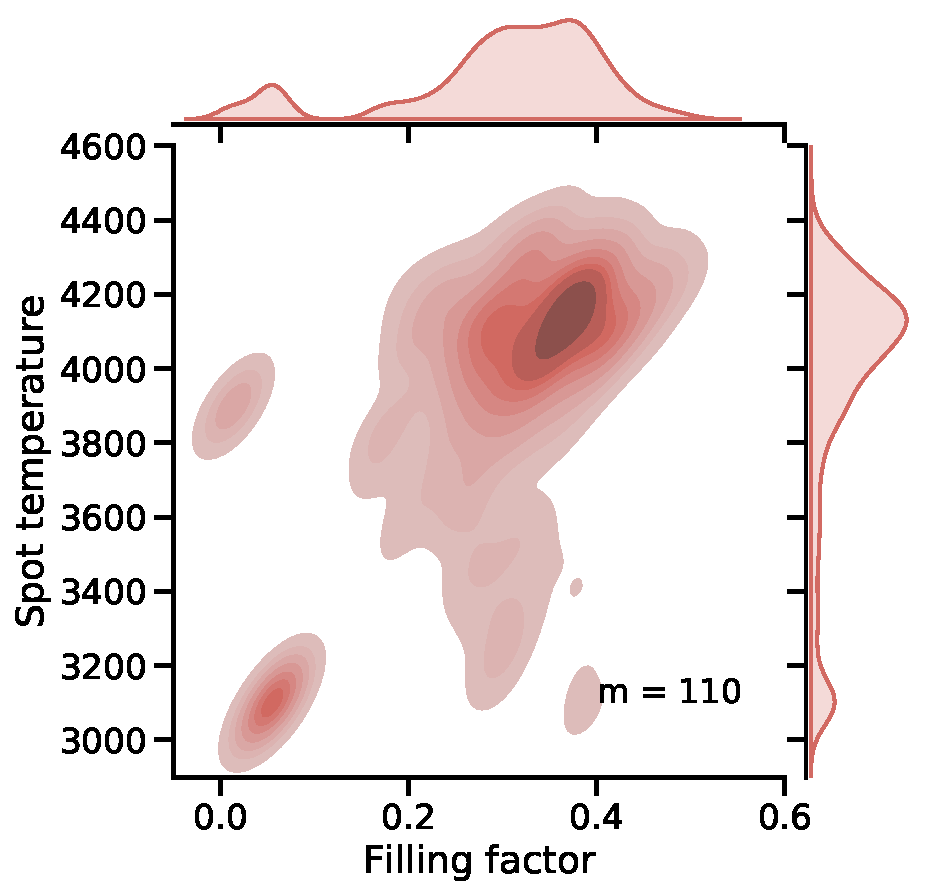
\includegraphics[width=2in]{figures/H_band_Tspot_fillingfactor_m110_new.pdf}} \\
     \subfloat{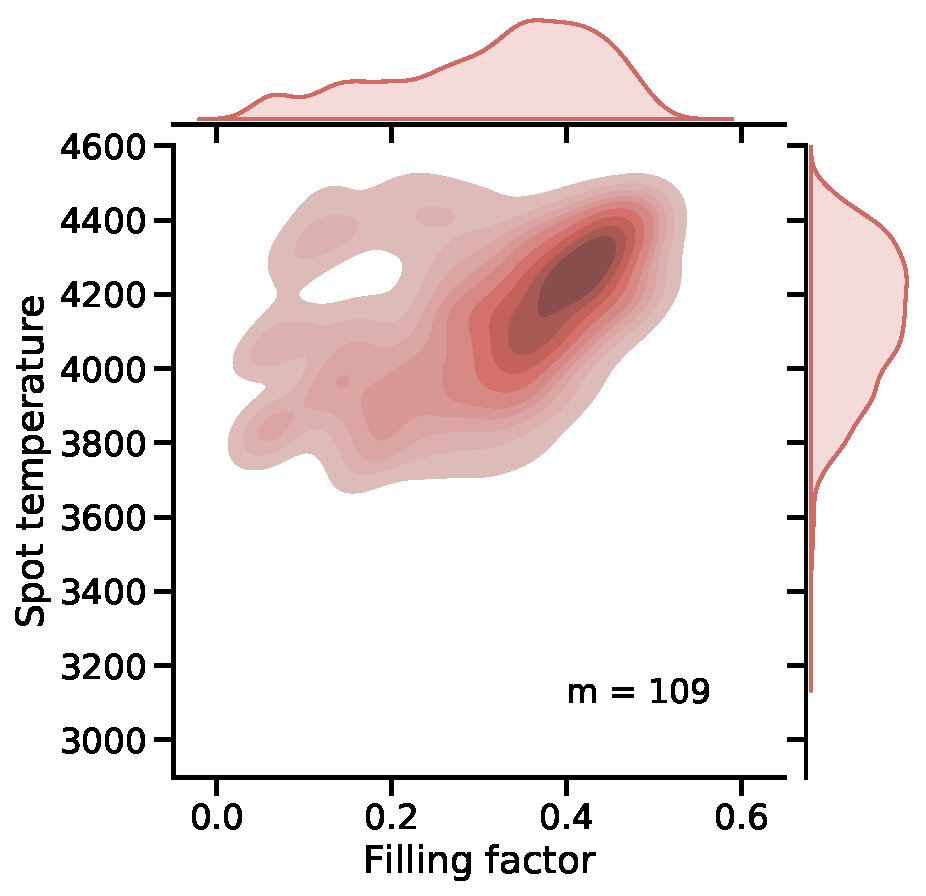
\includegraphics[width=2in]{figures/H_band_Tspot_fillingfactor_m109_new.pdf}} &
     \subfloat{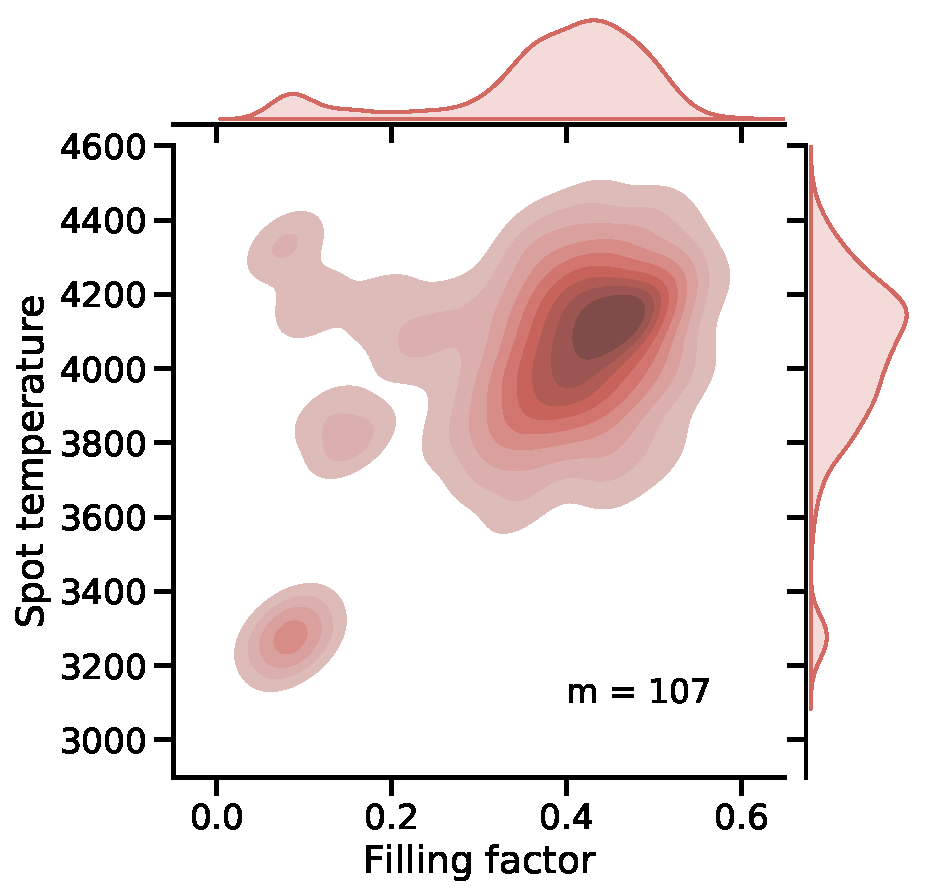
\includegraphics[width=2in]{figures/H_band_Tspot_fillingfactor_m107_new.pdf}} &
     \subfloat{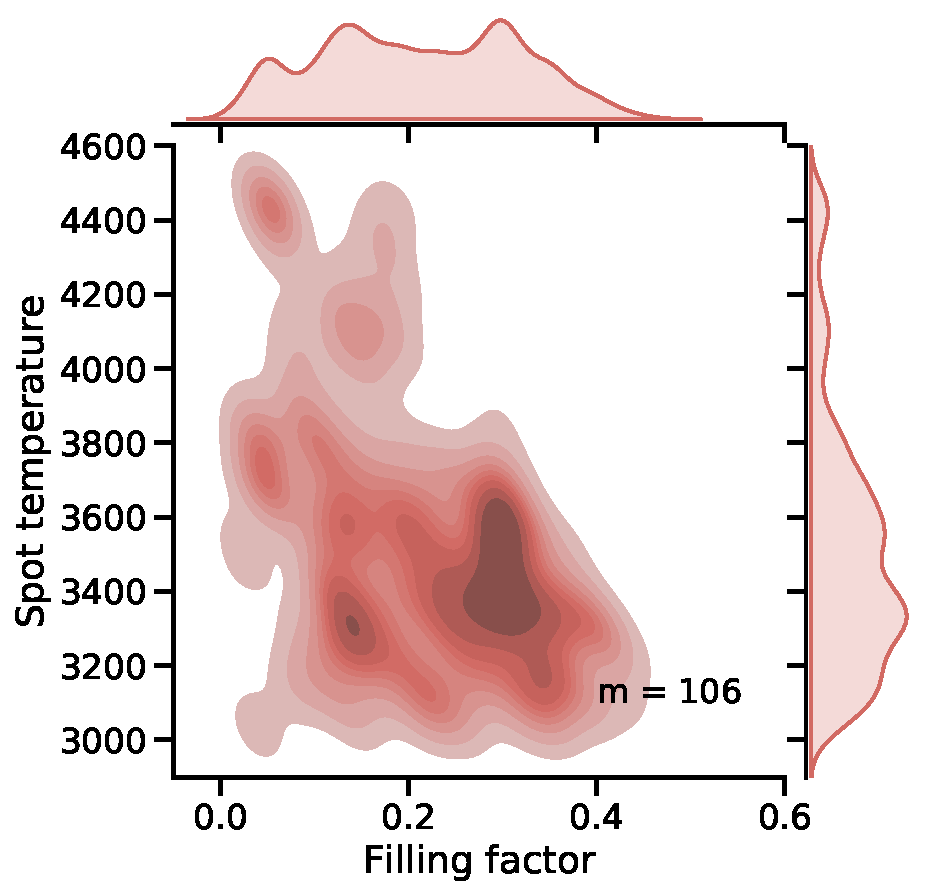
\includegraphics[width=2in]{figures/H_band_Tspot_fillingfactor_m106_new.pdf}}
   \end{tabular}
 \caption{2-dimensional distributions of filling factor and spot temperature for the nine accepted IGRINS orders for S1063, including 1000 samples of the emcee chains thinned by a factor of 10. Some orders demonstrate a stronger ability to constrain the spot characteristics than others, however all are consistent with the detection of a moderate covering fraction of spots. The median filling factor across these nine orders is $32 \pm 7$\% with a spot temperature of $4000\pm200$ K.}
 \label{fig:tspot_fillingfactor3x3}
 \end{figure*}

 \subsection{Comparison to evolutionary models of active stars}
 \label{sec:model_comparison}

\begin{figure*}[ht]
    \centering
    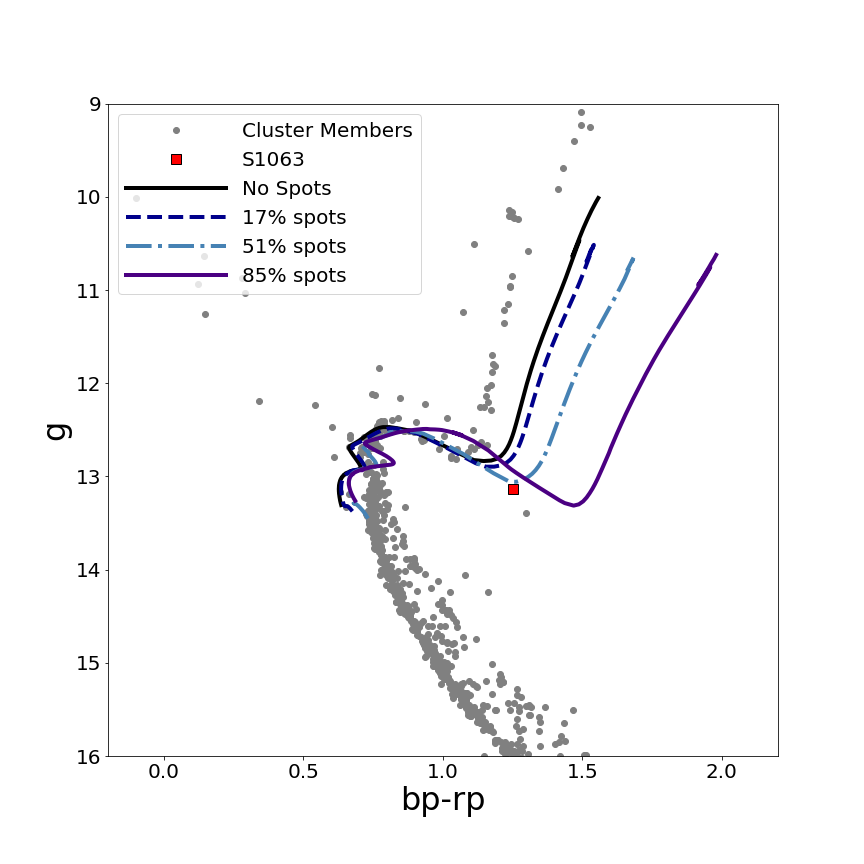
\includegraphics[width=0.45\linewidth]{figures/S1063_GaiaCMD.png}
    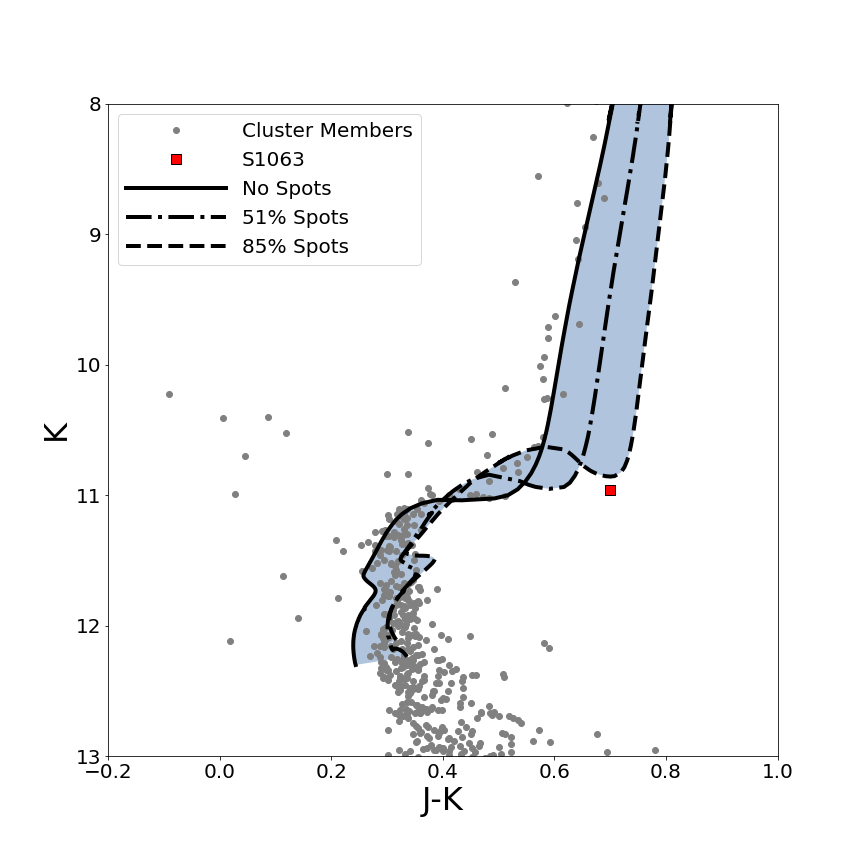
\includegraphics[width=0.45\linewidth]{figures/S1063_2MASS_CMD.png}
    \caption{On the left is a \textit{Gaia} color-magnitude diagram (CMD) that shows members of M67 (gray points) with SSG S1063 highlighted (red square). In comparison, we show SPOTS evolutionary tracks \citep{somers20} for a 1.3 \Msolar\ star (black lines). The shaded blue area between the tracks indicates the region occupied by stars with spot covering fractions between 0\% and 85\% according to the SPOTS models. On the right is a similar CMD using photometry from 2MASS.}
    \label{fig:CMDs}
\end{figure*}

Current theoretical modeling of active stars take several different approaches, including surface treatments of spots at non-zero temperatures that suppress convective energy transport \citep{somers20}, direct treatments of the interior magnetic field \citep{2013ApJ...779..183F}, and reduced mixing length models with non-emitting spots \citep{2007A&A...472L..17C}. Comparing observationally-constrained spot filling-factors with those from theoretical predictions can highlight current gaps in our knowledge, and therefore direct future studies.

Here, we compare the photometry of S1063 to spotted SPOTS evolutionary tracks \citep{somers20}. SPOTS models assume the presence of star spots inhibits local flux that must escape through ambient (non-spotted) regions of the stellar surface. To determine photometric conversions from the stellar structure models, all SPOTS evolutionary tracks adopt a two-temperature surface with a fixed ratio of spot to ambient temperature of 0.8. We use optical photometry from \textit{Gaia} and near-infrared photometry from 2MASS for this comparison, showing CMDs of M67 members compared to the shaded region in the each CMD populated by SPOTS tracks in Figure~\ref{fig:CMDs}. As expected, spotted sub-giant models appear redder and fainter than the sub-giant branch in both CMDs. We also show the unspotted SPOTS evolutionary track in each CMD as a black solid line. This unspotted model fits the typical subgiant branch of M67 in the 2MASS CMD, however this is not true when using Gaia photometry. In the Gaia CMD the unspotted SPOTS model has a more extended subgiant branch and redder giant branch than observed in the cluster. This discrepancy is not resolvable by changing cluster parameters (i.e. reddening, distance, turnoff mass, metallicity). It may be due to internal model physics (i.e. choice of mixing length) or an error introduced when calculating model colors in the Gaia bandpasses.

Photometry for S1063 from both Gaia and 2MASS is roughly consistent with the region populated by SPOTS evolutionary tracks. Generally, the spot covering fraction adopted from this model comparison would result in larger spot filling factors of approximately 50--85\%, depending on the photometry used, compared to the $32\pm7$\% filling factor found in this work. Another photometric comparison using a two-temperature SED fit of S1063 \citep{leiner17} finds a spot filling factor of 40\%, which is also in moderate disagreement with our results.



%The optical photometry is most consistent with a SPOTS model with a $\sim50\%$ spot filling factor, slightly higher than the $32\%$ we find from the spectroscopic deconvolution. The 2MASS photometry indicates an even larger filling factor, falling in between the 51\% and 85\% SPOTS models. We note that while the unspotted SPOTS evolutionary track (black line in Figure~\ref{fig:CMDs}) fits the turnoff of M67 well when using 2MASS photometry, the model has a more extended subgiant branch and redder giant branch compared to the \textit{Gaia} photometry. This discrepancy is not resolvable by changing cluster parameters (i.e. reddening, distance, turnoff mass, metallicity). It may be due to internal model physics (i.e. choice of mixing length) or an error introduced when calculating model colors in the Gaia bandpasses. Due to this improper calibration, the spot filling factor inferred from comparisons with the \textit{Gaia} photometry may be skewed towards lower spot filling factors. This could explain the higher spot filling factor inferred from the 2MASS photometry, where the unspotted models are a better fit to the cluster turnoff.



We believe that some of the discrepancy between our results and those predicted by the SPOTS models may be due to limitations of the SPOTS models as diagnostic tools for single sources. However, observational biases may also impact the filling factors determined through spectroscopic and photometric methods. The spectral decomposition technique used here is sensitive to larger spot filling factors \citep{gullysantiago17}, as long as the spots are of sufficient brightness to provide a significant spectral signature. We do detect a significant spot spectral signature in S1063, but we do not know if we are detecting the spectrum of the umbra or prenumbra. It is most likely that the penumbra is larger in area and warmer than the umbra for most stars \citep{1981ApJ...250..327V}. Spectral decomposition techniques are more sensitive to the warmer spot components and may therefore be constraining the prenumbra filling factor, which would be larger than the umbra filling factor. However, we do not know if the spot morphology of SSGs follows this assumption. If instead SSGs have a smaller ratio of prenumbra to umbra this spectral technique would under-sample the total spot coverage on the stellar surface.

Additionally, possible wavelength dependencies of spot size would lead to discrepant spot filling factors across photometric and spectroscopic determinations at different wavelengths. We note that photometry collected at different epochs can also impact the inferred photometric filling factor. Given our light curve analysis of S1063 we expect epoch-based filling factor uncertainties could be as large as $\sim$20\%, which could bring the two-temperature SED fit from \citet{leiner17} and our results into agreement.

A summary of the surface and stellar parameters for S1063 are given in Table~\ref{tab:s1063parameters}, comparing our work here with parameters for S1063 determined in \citet{mathieu03}, \citet{leiner17}, and the SPOTS model comparison above. As the closest SPOTS model depends on the comparison photometry used (see Figure~\ref{fig:CMDs}), the stellar parameters for both models are given.

We further discuss systematic uncertainties that may impact these discrepancies in Section~\ref{sec:uncertainties}, but fully resolving the complexities of photometric and spectroscopic constraints of spot filling factors likely requires careful photometric and atmospheric modeling of a multi-temperature stellar surface, which is beyond the scope of this paper.


\section{Discussion}
\label{sec:discussion}

The spot coverage fraction for S1063 determined in this work is consistent with the range of spot coverage seen on RS CVn of 30--40\% from measuring TiO band strength \citep{oneal96, oneal98, oneal04} and Doppler imaging \citep{hackman12}. This is further evidence that this SSG and likely other SSGs have high magnetic activity.

Strong magnetic fields and starspots reduce convective energy transport efficiency, which in turn alters theoretical evolutionary model tracks from their unspotted/non-magnetic counterparts \citep{2013ApJ...779..183F,somers15,somers15b,somers20}. Understanding the physical nature of the magnetic activity and the impact it has on stellar structure and evolution requires comparison of high-fidelity observations with these theoretical models.  An accurate HR diagram position requires determination of the effective temperature ($T_{\textrm{eff}}$) having accounted for spots, as well as the stellar luminosity.

\subsection{Effective temperature of spotted stars}
The conventional observational interpretation of $T_{\textrm{eff}}$ is difficult to apply to spotted stars, especially stars with variation in the spot covering fraction over time \citep{gullysantiago17}. Different methods of characterizing $T_{\textrm{eff}}$ complicate  comparisons between observations and theoretical models.

%Conventionally, a star is thought to have a single $T_{\textrm{eff}}$ that can be easily matched to  Conventionally, a spectrum can be interpreted as possessing a 1:1 mapping from its appearance to a $T_{\textrm{eff}}$-indexed template, which can be either model-based or observed.  We...

\citet{leiner17} fit the multi-band spectral energy distribution for S1063 with a single Castelli-Kurucz spectrum \citep{2003IAUS..210P.A20C} and find a best fit single-temperature $T_{\textrm{eff}}$ of 4500 K. With observational confirmation that S1063 is a spotted star, another interpretation is to calculate the surface-averaged $T_{\textrm{eff}}$:

\begin{equation}
T_{\textrm{eff}}^4 = f_{\textrm{s}} T_{\textrm{s}}^4 + (1 -f_{\textrm{s}}) T_{\textrm{amb}}^4 .
\end{equation}

where $f_{\textrm{s}}$ is the spot covering fraction, $T_{\textrm{s}}$ is the spot temperature, $T_{\textrm{amb}}$ is the ambient photosphere temperature. This surface-averaged temperature allows for comparisons to one-dimensional stellar evolution models motivated by the surface conditions of the star \citep{somers20}. With this method, at the time of the IGRINS observation the $T_{\textrm{eff}}$ of S1063 is $4900\pm100$ K. This temperature is inconsistent with the temperature determined via SED fitting in \citet{leiner17}, indicative of the discrepancies between the spectral and photometric constraints outlined in Section~\ref{sec:model_comparison}, although we note that the previous temperature of 4500 K is between the measured spot and ambient photosphere temperatures determined in this work.

Stars such as S1063, however, have observed surface-averaged $T_{\textrm{eff}}$ values that vary based on the spot covering fraction at the time of observation. We know from the variable light curve (Figure~\ref{fig:lightcurve}) that stars such as S1063 have differing spot covering fractions on opposite observable hemispheres of the star causing optical variability. For example, at the four-year light curve maximum S1063 had approximately 20\% spot covering fraction and a surface-averaged $T_{\textrm{eff}}$ (for the observed hemisphere of the star) of 5000 K. At the light curve minimum with a 45\% spot covering fraction the surface-averaged $T_{\textrm{eff}}$ for the observed hemisphere would only be 4700 K.

The true surface-averaged $T_{\textrm{eff}}$ includes the entire stellar surface. This should be constant over a thermal timescale, much longer than the four-year time frame in Figure~\ref{fig:lightcurve}, as is demonstrated by the constant mean flux level of 89.5\% compared to the maximum global flux. Observationally constraining the surface-averaged $T_{\textrm{eff}}$ requires either multi-epoch spectrum observations at both the light curve maximum and minimum, or a single observation at the mean flux level. The date of the IGRINS observation corresponds to a flux level of 91.2\% compared to the global maximum, suggesting that observed spot coverage is a reasonable proxy for the mean state of S1063. Therefore, we conclude that the total surface-averaged $T_{\textrm{eff}}$ of S1063 is consistent with the observed surface-averaged $T_{\textrm{eff}}$ of $4900\pm100$ K. We stress, however, that determining a single $T_{\textrm{eff}}$ value for spotted stars makes model comparisons exceedingly nuanced.


\subsection{Radius of S1063}
\label{sec:radius}

The radius of S1063 is encoded into data in three ways: via surface gravity-sensitive spectral lines, in the SED and HR Diagram position, and embedded within the $v\sin{i}$ measurement. Observationally constraining the radius of spotted stars would help model comparisons, especially in light of the single $T_{\textrm{eff}}$ nuances elaborated above.

Our weak constraints on surface gravity from the IGRINS spectra cannot meaningfully inform the radius. Previously determined SED-based photometric results suggest a radius of $R_{\star} = 2.8-3.4 R_\odot$ (see Table~\ref{tab:s1063parameters}). We elaborate on constraining the radius from $v\sin{i}$ here.
The stellar radius $R_{\star}$ contributes to the magnitude of the equatorial velocity $v_{\mathrm{eq}}$ for a given rotation rate and projected stellar inclination angle $i$:
\begin{eqnarray}
  v \sin{i} = \frac{2\pi R_{\star}}{P_{\mathrm{rot}}} \sin{i} \\
  R_{\star} \sin{i} = \frac{v \sin{i} \cdot P_{\mathrm{rot}}}{2 \pi} \label{rsini}
\end{eqnarray}

Our \texttt{Starfish}/IGRINS-derived $v\sin{i}=10.0 \pm 1.0 \; \mathrm{km\,s^{-1}}$ and \texttt{celerite}/K2 derived period $P_{\mathrm{rot}}=23.5 \pm 0.1$ constrain $R\sin{i} = 4.6 \;R_\odot$, with a formal statistical uncertainty of $\pm 0.5 \;R_\odot$.  For stars viewed at an inclination other than perfectly edge-on, the typical inferred stellar radius $R_{\star}$ must exceed $4.6 R_{\odot}$. If we instead adopt the optically-determined $v\sin{i}=8\; \mathrm{km\,s^{-1}}$ from \citet{mathieu03} the radius must exceed 3.7 $R_{\odot}$. In either case, this kinematically-inferred radius is inconsistent with the radius range determined through photometric studies. A two-temperature SED of S1063 adopting the minimum $R\sin{i}$ values is far too bright compared to observed photometry, suggesting that the $R\sin{i}$ limits here are biased to larger values in some way.

One possible source of this discrepancy is the spotted surface somehow alters the assumptions behind Equation \ref{rsini}. Possible astrophysical uncertainties that could potentially bias the $v\sin{i}$ for heavily spotted sub-giants include the adopted limb-darkening prescription, micro- or macro-turbulence, and Zeeman broadening. Additionally, the observed period could be biased via differential rotation combined with starspots constrained to either high or low latitudes, starspot evolution timescales similar to the rotation period, and aliasing from regularly-spaced longitudinal surface symmetries. The magnitude and/or direction of these period biases are generally uncertain. We note that the other SSG in M67, S1113, also has an anomalously-large $R\sin{i}$ value determined from $v\sin{i}$ \citep{mathieu03}, suggesting that perhaps the surface conditions of SSGs cause spectral broadening such that the standard $v\sin{i}$ measurement is not truly a measure of the stellar rotation velocity. A campaign of intense doppler-imaging-style observations could act to disentangle some of these uncertainties in the future, though such a campaign would require extreme spectral resolution in order to resolve surface structures given the relatively low apparent $v\sin{i}$.

%We consider for the moment a hypothetical perfectly edge-on orientation.  The kinematically derived radius exceeds its photometric counterpart by 2.6$\,\sigma$, an ostensible tension for these two disparately-sourced estimates. However, we consider the possibility that the star is so profoundly spotted as to alter the assumptions that lead to Equation \ref{rsini}.  At least four sources of unaccounted-for astrophysical uncertainties can conceivably bias the derived $v\sin{i}$ for heavily spotted sub-giants.  The limb-darkening prescription, unaccounted for Zeeman broadening, micro- or macro- turbulent velocity, and the latitudinal segregation of starspots all act to modulate the mapping from observed line profile to inferred $v\sin{i}$.  On the other hand, the period can be systematically biased in three significant ways: differential rotation combined with latitudinal starspot segregation, starspot evolution on timescales comparable to the rotation period, and aliasing from regularly-spaced longitudinal surface symmetries.  The aggregate magnitude and/or direction of these systematic biases is generally uncertain, and even the rank order of which bias predominates may defy the routine assumptions applied to modestly spotted stars like the Sun.  We therefore attribute the apparent tension in our radius uncertainties to these epistemic uncertainties with magnitudes comparable to or greater than the formal statistical uncertainties.  A campaign of intense Doppler-Imaging-style observations could act to disentangle some of these uncertainties in the future, though such a campaign would require extreme spectral resolution in order to resolve surface structures given the relatively low apparent $v\sin{i}$.

%-Now there is tension with the colors of the SPOTS models, but colors of spots are weird. The lower spot coverage models predict bluer colors than observed. Perhaps some chromospheric component? This is probably fine.

%-Perhaps demonstrates a need for a dual modeling approach of surface treatment with internal structure changes and comparing against a larger sample of stars




\subsection{Additional sources of systematic uncertainty}
\label{sec:uncertainties}
We assume a two-temperature stellar surface to derive our estimates for spot filling factor and effective temperature.  In reality, this star---and most active stars more generally---must exhibit a range of apparent surface features attributable to umbra, penumbra, faculae, chromospheric emission, and other phenomena unaccounted for in this work \citep{berdyugina05, 2009A&ARv..17..251S}. These phenomena all have different temperatures and wavelength-dependent flux contrasts with the ambient photosphere.

Our near-IR spectral technique is most sensitive to detecting a ``sweet-spot'' in starspot contrast: cool enough to exhibit a spectrum that is qualitatively distinct from the ambient photosphere, but not so cool as to possess vanishing specific intensity.  So for example, our technique might readily perceive the penumbra of the starspot, while ignoring the much cooler and darker umbra flux contribution \citep{1981ApJ...250..327V}.  This bias would lead our technique to systematically underestimate the total starspot coverage, rendering our claimed estimate as a lower limit.  On the other hand, faculae and plage act to add a hotter-than-average surface component. Our two-component model cannot accurately account for the coexistence of spots and faculae with an ambient photosphere \citep{1998A&A...329..747S}. Specifically, faculae may act to either increase or decrease starspot coverage estimates insofar as they alter the determined ambient photosphere temperature  \citep{2019AJ....157...11W}. The existence of large and hot faculae can be ruled out to some extent by the fact that they would dominate the temperature determination in visible wavelength spectra.  The adequate agreement in ambient temperature derived from visible \citep{mathieu03} and near-IR spectra of S1063 in this work suggests that faculae may be negligible.  Chromospheric emission should mostly perturb individual lines that are known to be chromospherically active, such as Hydrogen lines.  Our IGRINS-based technique analyzed the majority of the $H$-band with whole-spectrum fitting, where such chromospherically active lines would have negligible impact.

Our reliance on \texttt{PHOENIX} synthetic spectra adds a model-dependent systematic to our entire approach.  The unavailability of a large number of spot-free high-precision high-resolution empirical template spectra across all of $H$-band demands the use of these models in order to compare to IGRINS data.  The ability of such synthetic spectra to resemble starspots remains an unknown.  We can examine fit residuals to explore the performance of the synthetic spectra by comparing the purple two-component composite spectrum to the gray IGRINS spectrum in Figure \ref{fig:IGRINS_spectra3x3}. We see that the observed IGRINS spectrum has lines that do not appear in the model, and the model has lines that do not appear in the observed spectrum. To some extent, the imperfect fitting of the synthetic spectra to our IGRINS spectra must be causing a systematic uncertainty.  The Gaussian process ``Global Kernels'' employed in \texttt{Starfish} account for some degree of correlated data-model residual mismatching.  We did not employ the ``Local kernels'', which cause a 30 K systematic bias in comparable quality spectra of WASP-14 also compared to the \texttt{PHOENIX} models \citet{czekala15}.  We therefore assign at least a 30 K systematic bias in our temperature estimates based on the prospect of individual line outliers polluting our fit residuals.  We co-assign a coarse estimate of 100--200 K to so-called ``label noise'', associated with the alignment of a best fit \texttt{PHOENIX}-provided temperatures and an unseen ground-truth label for the ``True'' temperature of the spots. New studies of the Sun based on DKIST may offer the best future avenue for testing such assumptions and refining the ability to distinguish starspot emission from ambient photosphere.



%\subsection{Starspots as confounding factors}
%Mass, age, and metallicity uniquely map a main sequence star to its HR diagram position.  A fourth factor---rotation---confounds this mapping in as-yet-unknown ways.  Rotation might enhance spread in HR diagram positions (cite XX Davenport, Douglas?), with the most conspicuous spreads in the pre-main sequence regime (cite XX Covey, Stauffer).  Spreads in the HR diagram offer clues to the consequences of rotation.  Increased rotation heightens the magnetic dynamo strength and concomitant surface magnetic field.  These magnetic fields suppress convective efficiency, meaning the star must increase in size at a lower effective temperature to allow the same amount of internal energy to escape (cite XX Feiden): rotating stars become bigger and cooler than their non-rotating counterparts (cite XX Somers).  The interplay of rotation, dynamo, and surface fields remain an active area of research, with bright prospects for a unified theory involving the degree of magnetic complexity parameter (cite XX Garraffo).

%Surface magnetic fields offer two key observational manifestations.  The Zeeman Effect splits spectral line levels in magnetic-sensitive atomic transitions (cite XX Johns-Krull).  Starspots induce stellar surface inhomogeneities that can be seen in the modulation of

%The story in the post-main sequence is less clear.  Angular momentum transport governs rotation  as stars evolve over orders of magnitude in size.

%\item Conceivable geometries with circumpolar active longitudes, or migrating active latitudes
%\item Biases introduced if we assume a spot-free model


\section{Conclusions}
\label{sec:conclusions}

The impact of magnetic activity on stellar evolution is a quickly developing field in stellar astrophysics. SSGs serve an important sample for furthering our knowledge, as they exhibit dramatic offsets from typical stellar evolutionary pathways \citep{geller17, leiner17}.


We use a combination of a light curve analysis and a near-IR spectral decomposition technique to constrain the starspot filling factor of SSG S1063 in open cluster M67. Previous work suggested that the underluminosity apparent in SSGs could be caused by inhibited convective energy transport due to high magnetic activity \citep{leiner17}. Constraining star spot filling factor is a helpful proxy for determining stellar magnetic activity, and this spectral decomposition technique allows for constraints on a much larger sample of stars than can be studied with Doppler Imaging or interferometry.

We find a spot filling factor for S1063 of $32\pm7$\% at the time of the IGRINS observation. By combining this constraint with the variability seen in the four-year light curve we determine that this is approximately the mean state of the star over this four-year time period, with a minimum and maximum spot covering fraction of 20\% to 45\%, respectively. Importantly, this technique reveals that the maximum light during this time period did not correspond to an un-spotted star. This spot filling factor is consistent with those determined for RS CVn stars through other methods, suggesting that SSGs are another type of active giant star binary systems.

The spot filling factor found here is generally less than the filling factor found through indirect photometric comparisons. It is possible that different sensitivities to umbra or prenumbra features of spots, wavelength dependencies in detected spot size, or differences in the observed hemisphere of the star across different epochs of observation could all result in different determinations of spot filling factor between spectroscopic and photometric techniques. However, the state of current stellar activity theoretical models makes direct comparison difficult. We encourage future work in careful conversion between stellar structure models and observational signatures, including spectroscopic templates, to help resolve these apparent discrepancies. %The source of the discrepancies between spectroscopic and photometric methods is not entirely clear, but may be due to different sensitivities to umbra or prenumbra features of spots, wavelength dependencies in detected spot size, or differences in the observed hemisphere of the star across different epochs of observation.

We find that reporting a single ``$T_{\mathrm{eff}}$" for active spotted stars is a confusing concept at best, and can lead to unclear or possibly incorrect observational and model comparisons. The surface-averaged $T_{\mathrm{eff}}$ derived from our results is not consistent with a single SED-fit temperature for S1063. Additionally, determining the surface-averaged $T_{\mathrm{eff}}$ for S1063 would vary from 4700 K to 5000 K depending on the epoch of observation, as only one hemisphere of the star can be observed at a time. We encourage future work in this area to be as explicit as possible when reporting temperatures for active stars to enable the most accurate comparisons between observational and theoretical efforts.

There is still much we do not understand about spot morphologies, the observational biases that impact our assumptions about spot filling factors, and how measurements of the stellar surface can be connected to the internal structure of the star. Focused studies such as these serve as important benchmarks for technique development, but larger studies of starspots on active stars are necessary to explore the suggested discrepancies between different observational methods of determining spot filling factors. These larger studies would also serve as important test samples for observational and theoretical comparisons to untangle the impact of stellar activity on stellar evolution.



\clearpage
\pagebreak


%\appendix
%\section{Appendix heading}
%\label{methods-details}
%Placeholder text

\begin{acknowledgements}

%ADS
This research has made use of the NASA Astrophysics Data System.
%IGRINS
This work used the Immersion Grating Infrared Spectrometer (IGRINS) that was developed under a collaboration between the University of Texas at Austin and the Korea Astronomy and Space Science Institute (KASI) with the financial support of the US National Science Foundation under grant AST-1229522, of the University of Texas at Austin, and of the Korean GMT Project of KASI.
%Kepler
This paper includes data collected by the Kepler mission. Funding for the Kepler mission is provided by the NASA Science Mission directorate.
% MAST
Some of the data presented in this paper were obtained from the Mikulski Archive for Space Telescopes (MAST). STScI is operated by the Association of Universities for Research in Astronomy, Inc., under NASA contract NAS5-26555.

%gaia
This work has made use of data from the European Space Agency (ESA) mission
{\it Gaia} (\url{https://www.cosmos.esa.int/gaia}), processed by the {\it Gaia}
Data Processing and Analysis Consortium (DPAC,
\url{https://www.cosmos.esa.int/web/gaia/dpac/consortium}). Funding for the DPAC
has been provided by national institutions, in particular the institutions
participating in the {\it Gaia} Multilateral Agreement.

\end{acknowledgements}

\facilities{Smith (IGRINS), Gaia, ASAS}

\software{  pandas \citep{mckinney10},
  emcee \citep{foreman13},
  matplotlib \citep{hunter07},
  numpy \citep{2020NumPy-Array},
  scipy \citep{2020SciPy-NMeth},
  ipython \citep{perez07},
  starfish \citep{czekala15},
  seaborn \citep{waskom14},
  lightkurve \citep{geert_barentsen_2019_2565212}}

\clearpage

\bibliography{ms}

\end{document}
